This exercise focuses on red eye removal from a picture (in this case, the picture on \autoref{fig:ex4-before}).
The specified sequence of steps is to start out by computing a score for each pixel that estimates the likelihood of that pixel belonging to a read eye (high score more likely).
The score is known as normalized cross-correlation and is expressed naturally as a stencil operation.
This score has already been computed in the exercise and the next step is therefore to sort these scores in ascending order (likelihood) effectively.
The final step is to reduce the redness of the highest scoring pixels and this can be performed using simple map operations.
As stencil and map operations have already been worked on in previous exercise, the focus of this exercise is to perform the sorting efficiently.
The result of the red eye removal can be seen in \autoref{fig:ex4-after}.
\begin{figure}[ht]
	\centering
	\begin{subfigure}{.5\textwidth}
		\centering
		\fbox{
			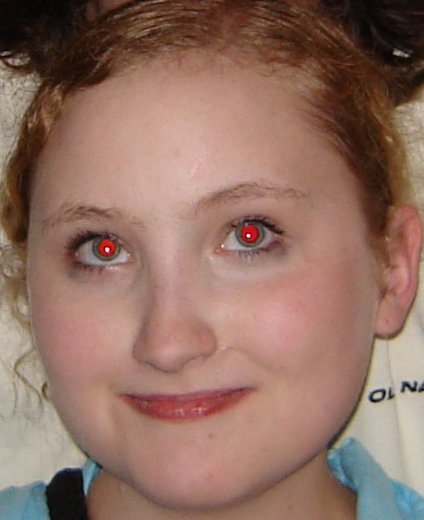
\includegraphics[width=0.4\textwidth]{figs/exercises/ex4/red_eye_effect_5.jpg}
		}
		\caption{Before}
		\label{fig:ex4-before}
	\end{subfigure}%
	\begin{subfigure}{.5\textwidth}
		\centering
		\fbox{
			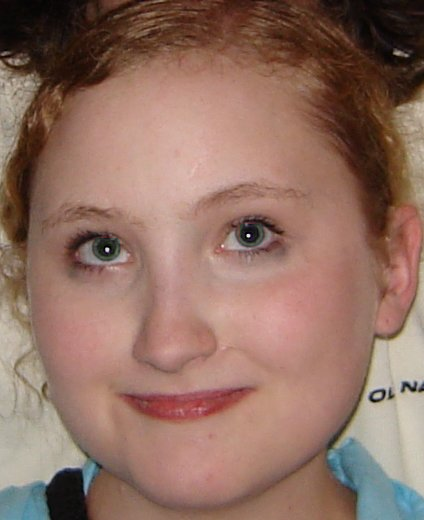
\includegraphics[width=0.4\textwidth]{figs/exercises/ex4/HW4_output.png}
		}
		\caption{After}
		\label{fig:ex4-after}
	\end{subfigure}
	\caption{Picture before and after red eye removal}
	\label{fig:ex4}
\end{figure}

The actual exercise is to implement a parallel radix sort.
To compute the sort, a lot of work has to be done (the actual source code can be seen in \cite{exercises}.)
The following sequence of techniques are performed for every bit of the values to sort (32bit values in this exercise).

% rewrite this

For every bit, starting a LSB, a histogram of the number of occurrences of each digit (0 or 1)
Exclusive prefix sum scan of histogram
predicate kernel (return vector with 1 for all ones and a vector with 1 for all zeros)
Exclusive prefix sum scan of predicates, exclusive prefix sum scan of incr values and add kernel at the end
move kernel, move to position if predicate is one
swap input and output (out of order sort)

\autoref{fig:ex4-radix-sort}

\begin{figure}[ht]
	\centering
	\fbox{
		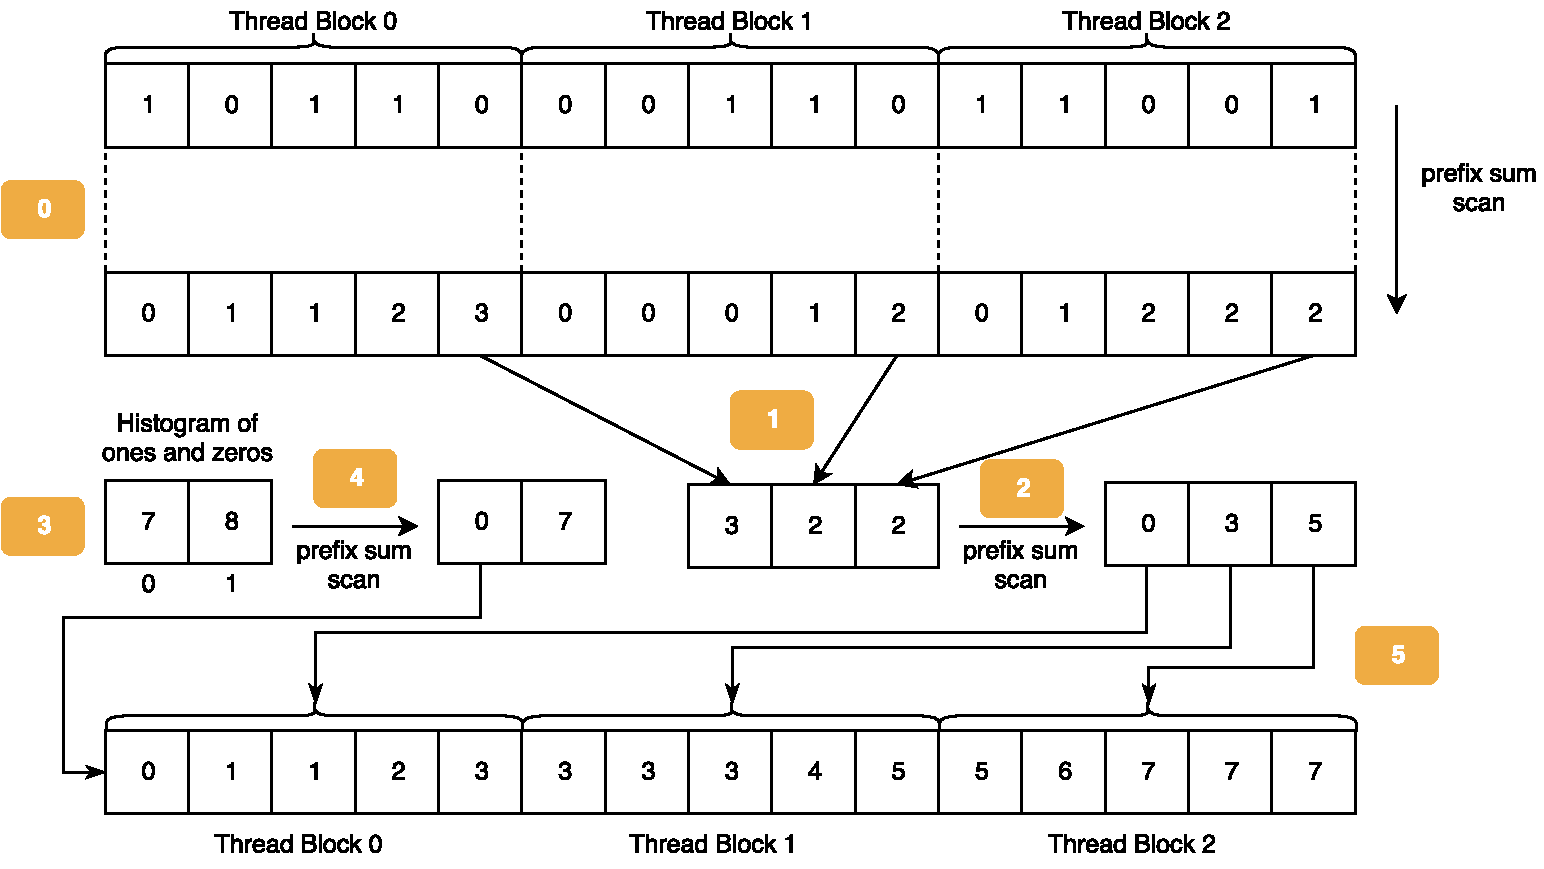
\includegraphics[width=1.0\textwidth]{figs/programming-model/ex4-radix-sort.pdf}
	}
	\caption{Exercise 4 radix sort implementation}
	\label{fig:ex4-radix-sort}
\end{figure}








